\subsection{MM/GB(PB)SA}\label{subsection:pbsa-theory}
    \paragraph{}
        \gls{acr:pbsa}\cite{Kollman2000CalculatingModels} or \gls{acr:gbsa} are computational methods that attempt to estimate the free energy of binding between two systems. It uses an implicit solvent model, in combination with a molecular mechanics force field and an understanding of the conservation of energy to estimate the Gibb's free energy of binding between a protein and ligand system.

    \paragraph{}
        \gls{acr:pbsa} and \gls{acr:gbsa} are often used interchangeably and the relative performance of both methods can be system dependant with the difference between the two being from the implicit solvent method used. \gls{acr:pbsa} uses the Poisson-Boltzman solvent model to describe the solvation energies of each model where as \gls{acr:gbsa} uses the generalised born solvent model.
        
\begin{figure}[H]
    \centering
    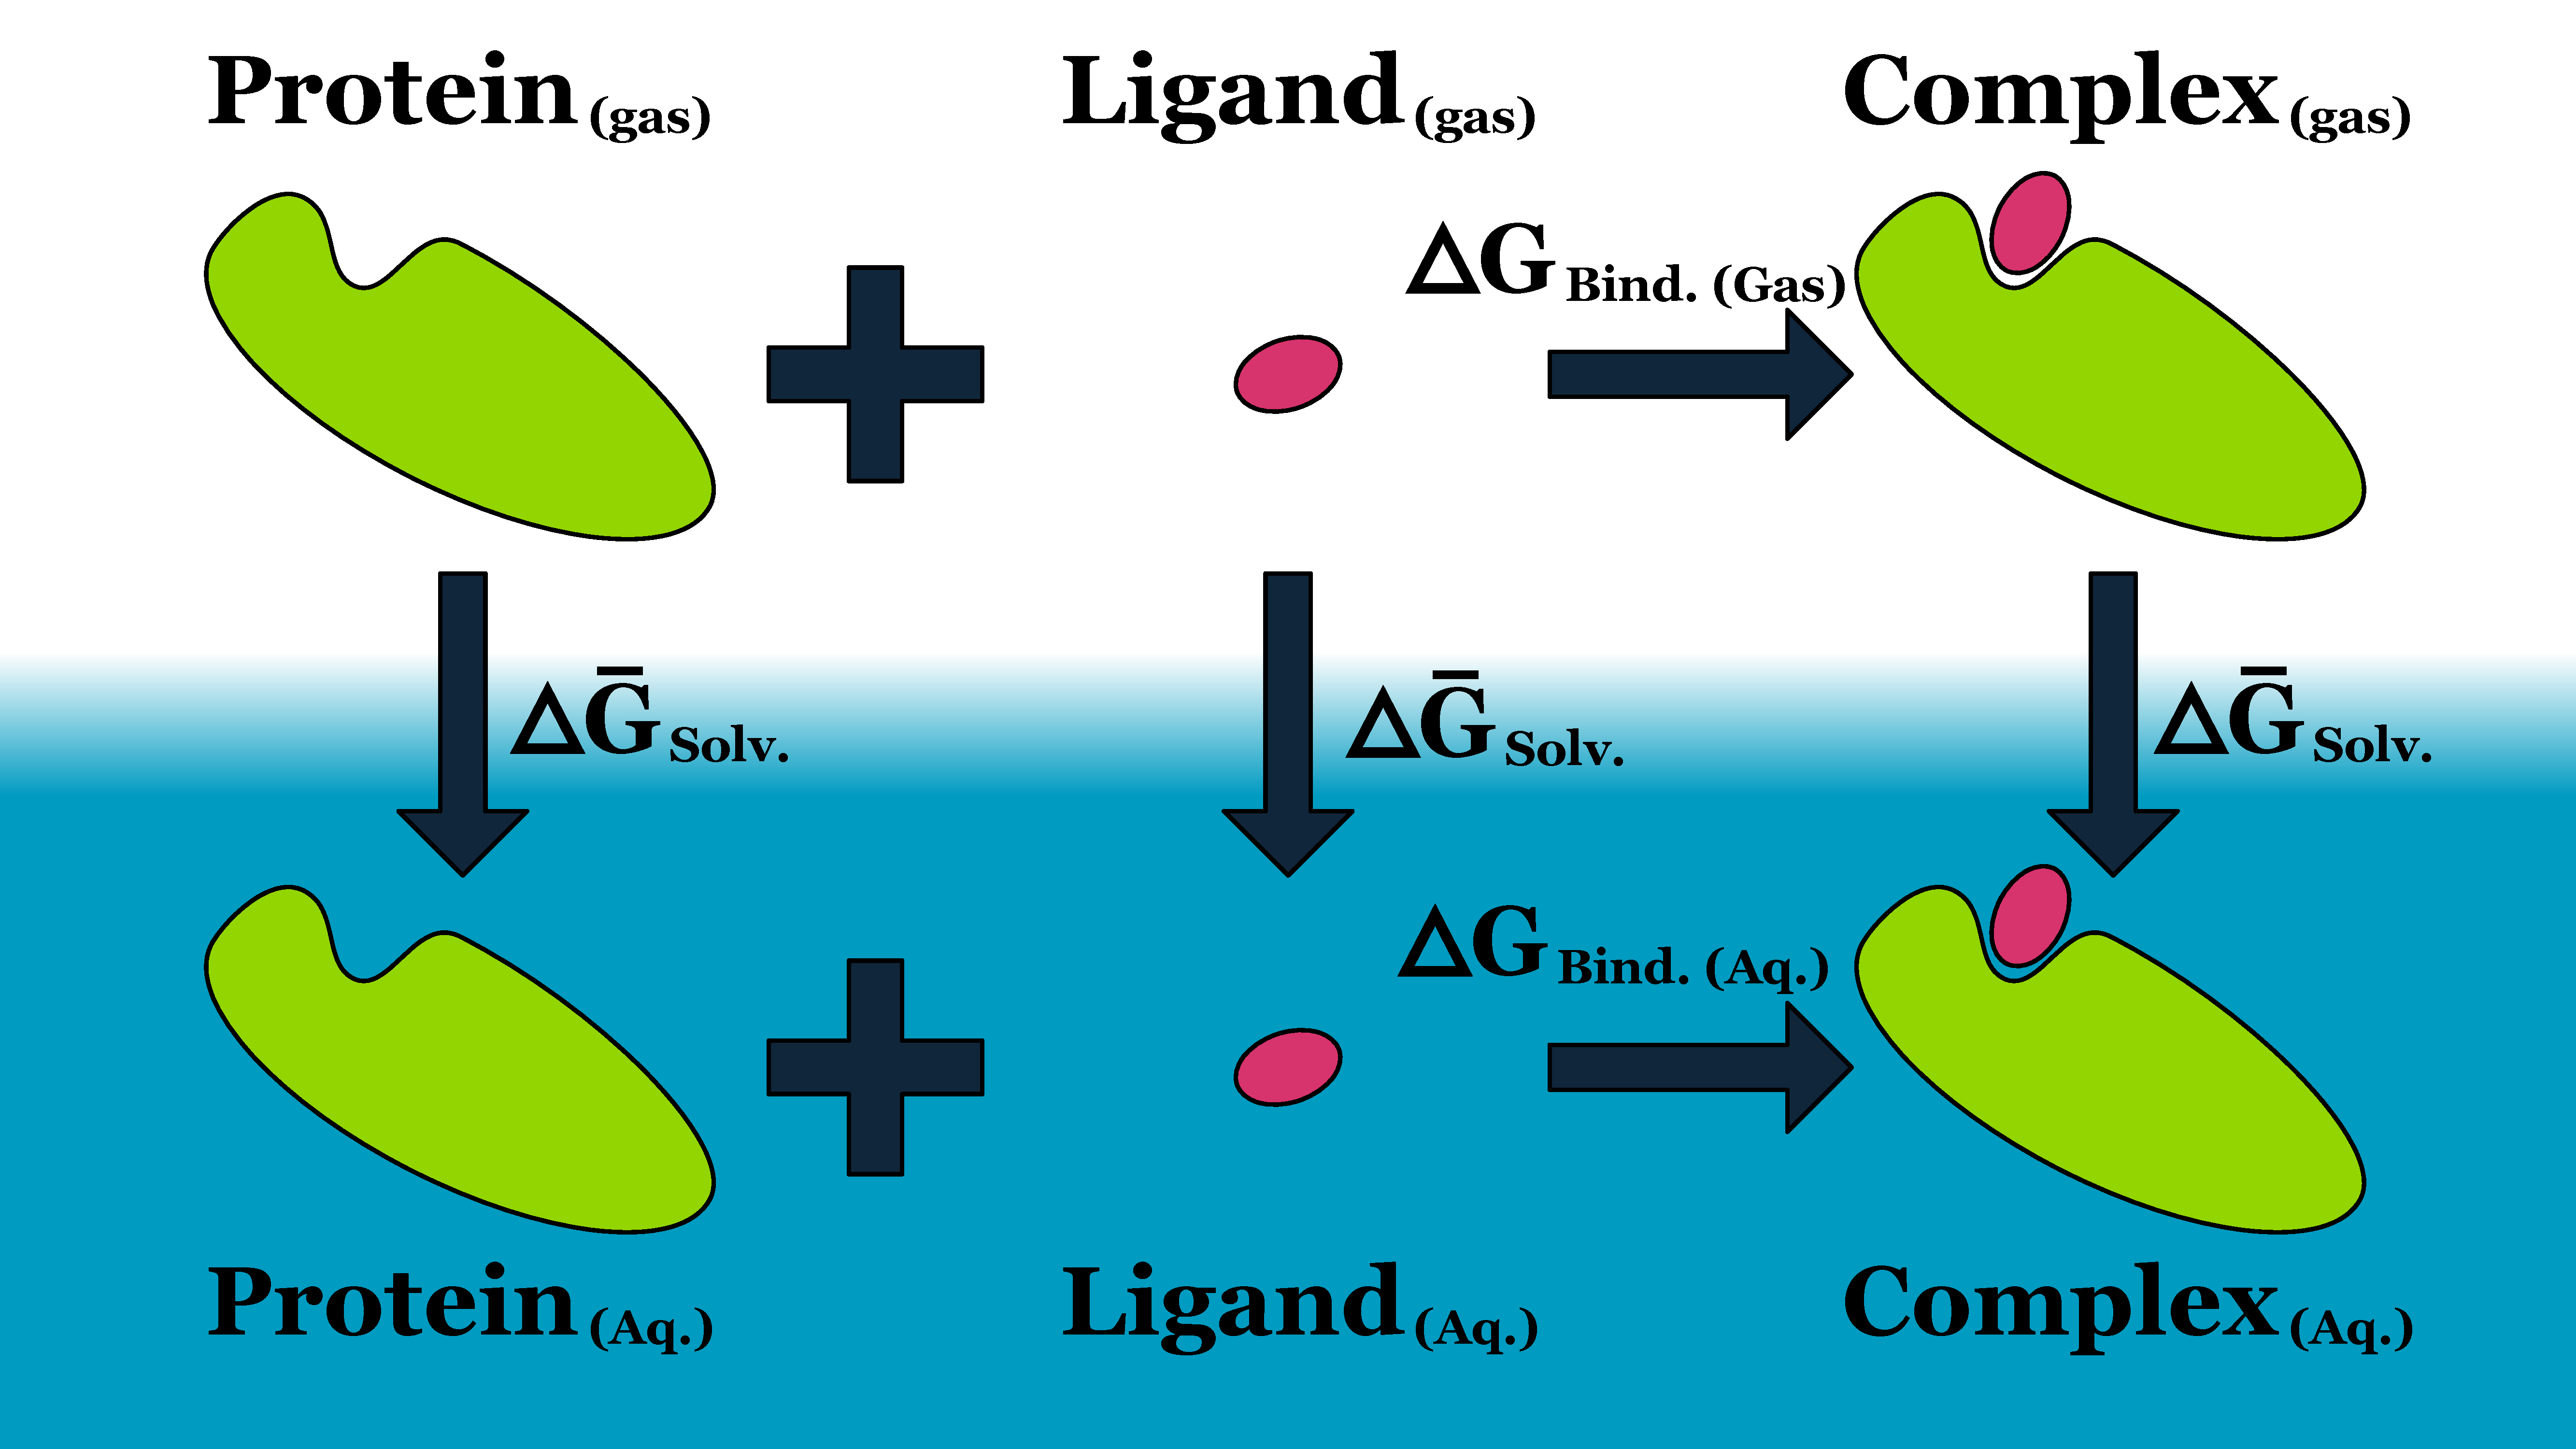
\includegraphics[width=\textwidth]{Graphics/Theory/gbsa.pdf}
    \caption{A visual representation of the MM/PB(GB)SA thermodynamic cycle.}
    \label{fig:mmpbsa}
\end{figure}

    \paragraph{}
        The \gls{acr:gbsa} method requires a traditional molecular dynamics simulation and uses post-processing to calculate the free energy, $\bar{G}$, of the structure through removal of the explicit waters and counter ions.  The free energy of the structure is calculated using equation \ref{eq:G}.

    \begin{equation}\label{eq:G}
        \bar{G} = E_{MM} + G_{PBSA} -TS_{MM}
    \end{equation}

    \paragraph{}
        Where $E_{MM}$ is the molecular mechanical energy which is taken from the forcefield used within the simulation (equation \ref{eq:EMM}).

    \begin{equation}\label{eq:EMM}
        E_{MM} = E_{bond} + E_{angle} + E_{tors} + E_{vdw} + E_{elec}
    \end{equation}

    \paragraph{}
        $G_{PBSA}$ is the solvation free energy of the structure, which uses the implicit solvent model in combination with a simple surface area term to estimate the solvation energy. $TS_{MM}$ is the entropy and can be estimated using quasi harmonic analysis of the trajectory, or normal-mode analysis.
        
    \begin{equation}\label{eq:GBSA}
        \Delta G_{bind} = \Delta \bar{G}_{complex} - \Delta \bar{G}_{prot.} - \Delta \bar{G}_{lig.}
    \end{equation}